\section{What it costs, and at what budget it wins}
\label{sec:cost}

Every result in \S\ref{sec:reward} is indexed by \emph{iteration}, which is not a fixed unit of
spend. A $\Kf$ optimizer step simulates five extra utterances per candidate --- eight candidates
per prompt, one patient API call and one policy generation per utterance --- so an iteration of
$\Kf$ buys strictly more compute than an iteration of $\Kz$, and reporting only the
matched-iteration result would flatter the lever. This section reports it on the axis that
actually constrains a practitioner.

\textbf{The multiplier.} Across the settled iterations 3--10 a $\Kf$ optimizer step costs a median
$\mathbf{1.92\times}$ a $\Kz$ step (range $1.83$--$2.18$; iterations 1--2 ran at a smaller
look-ahead sub-batch and are excluded). Over the whole run the two arms cost $51.205$ and $27.906$
GPU-hours --- $\mathbf{1.835\times}$, slightly below the per-step figure because generation
outside the optimizer loop is shared. GPU-hours are \emph{reconstructed} from per-step artifact
timestamps rather than read from a timing field, because the metadata's elapsed-time fields are
per-process and undercount any iteration that crashed and resumed --- in one case by nearly a
factor of two (Appendix~\ref{app:repro}).

\begin{figure}[t]
\centering
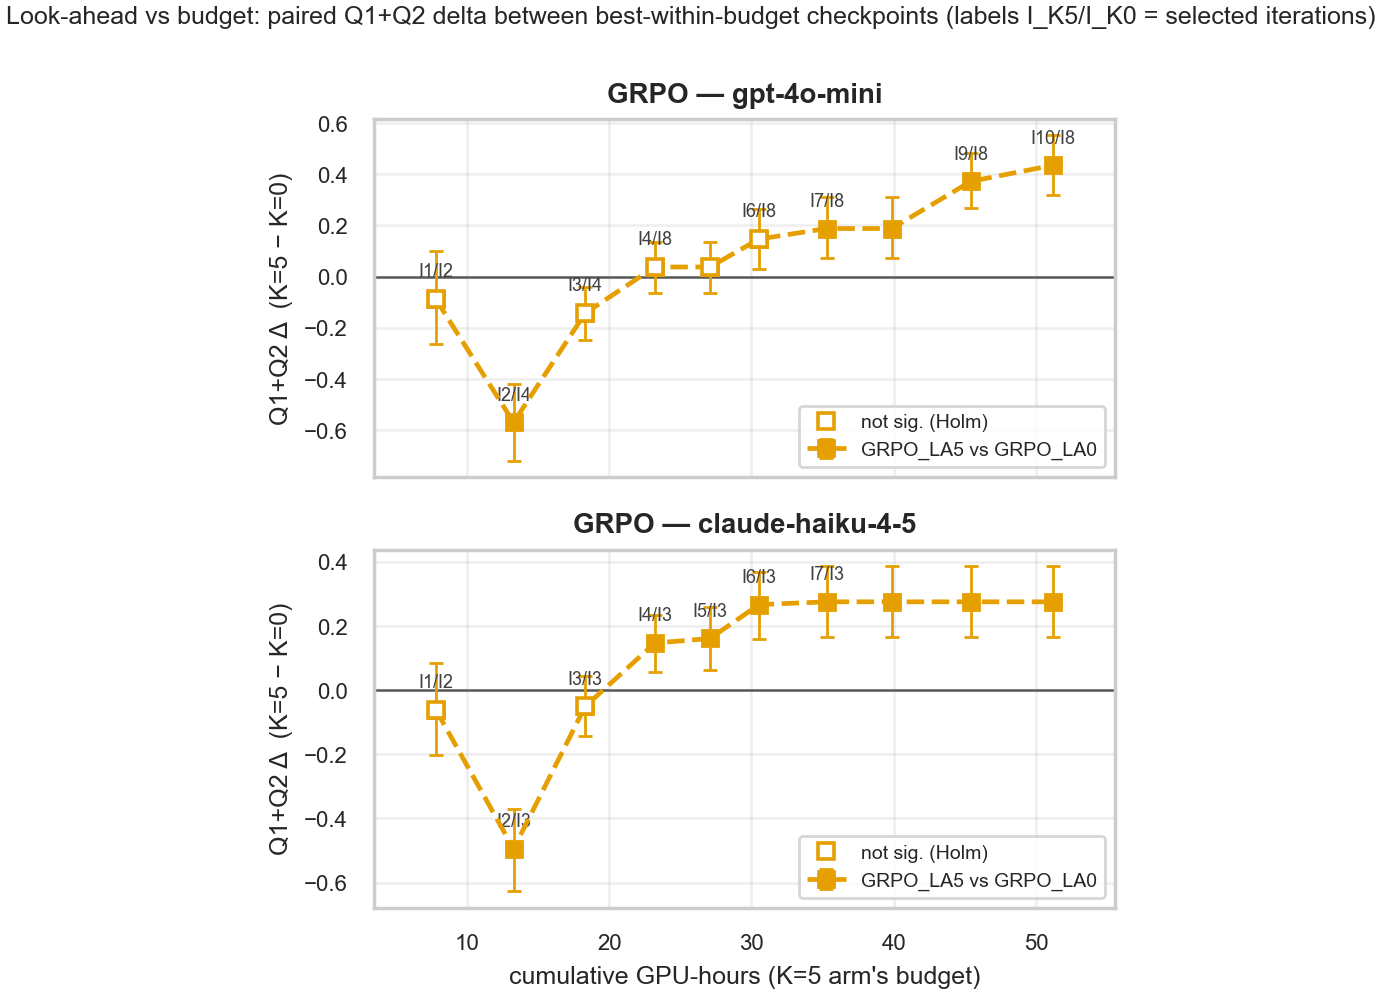
\includegraphics[width=0.55\textwidth]{figures/budget_sweep_grpo.png}
\caption{Paired Q1+Q2 delta ($\Kf - \Kz$, so \emph{up is look-ahead winning}) between the best
checkpoints reachable within a given GPU-hour budget, under each grader. Hollow markers did not
clear Holm; labels name the selected iterations. Below ${\sim}18$ GPU-hours look-ahead is behind;
it crosses zero near $23$ under both graders --- already Holm-significant there under the held-out
judge, from $35$ under the training oracle.}
\label{fig:budget}
\end{figure}

\textbf{The lever's sign is a function of budget.} Matching on budget rather than iteration
reverses the verdict at small budgets and confirms it at large ones (Figure~\ref{fig:budget}).
Under the training oracle: at $18.31$ GPU-hours look-ahead is \emph{behind} by $-0.143$
($\dz\,-0.276$); at $23.21$ it has drawn level ($+0.038$, n.s.); its first Holm-significant win is
at $35.29$ GPU-hours ($+0.188$, $\dz\,0.310$, $p_{\text{holm}}\,.020$); and at the common $51.20$
GPU-hour budget it leads by $+0.435$ ($\dz\,0.743$, $p_{\text{holm}}<.001$). The held-out judge
crosses at the same rung but is Holm-significant there immediately ($+0.147$, $\dz\,0.331$,
$p_{\text{holm}}\,.012$ at $23.21$) --- it moves the significance forward, not the crossover. The
practical statement is therefore conditional, and we state it that way: \textbf{under roughly 20
GPU-hours, spend the budget on more $\Kz$ iterations; past roughly 35 (23 by the held-out judge),
spend it on look-ahead.} Take the sweep, not any one rung --- the rungs are not independent, since
each compares the best checkpoint each arm can reach by that budget.

\textbf{The win survives honest model selection.} Choosing ``the best checkpoint'' on the same
grader that then evaluates it is optimistic. Repeating the $51.2$ GPU-hour comparison under all
four combinations of selecting grader $\times$ evaluating grader --- including the two \emph{honest}
cells where selection and evaluation use different graders --- look-ahead wins in \textbf{4 of 4},
with $\Delta$ from $0.256$ to $0.435$ and every $p_{\text{holm}} < .001$. The MI-inconsistency
advantage survives the budget axis as well: at $51.2$ GPU-hours with checkpoints selected on Q1+Q2,
MICI is $0.210$ for $\Kf$ against $0.535$ for $\Kz$ ($\dz\,-1.129$, lower better) --- look-ahead is
not buying reward by converting compute into a better-hidden hack. \S\ref{sec:behaviour} makes that
case from the transcripts rather than from the grader.
